\scanpage{80}
% archive sheet number: 79
% margin note written slanted; top edge clips the first line.
\margin{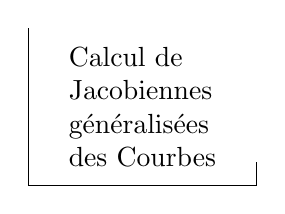
\begin{tikzpicture}\node[align=left] (t) {\unsure{Calcul de}\\Jacobiennes\\\unsure{généralisées}\\des Courbes};\draw (-1.45,1)--(-1.45,-1)--(1.45,-1)--(1.45,-.7);\end{tikzpicture}}
% D1, upper spectral-sequence scheme; the two inner terms are circled.
\diagram{\begin{tikzcd}[ampersand replacement=\&,column sep=large,row sep=small]
\text{\uuline{$\operatorname{Ext}$}}^*(\unsure{\mathscr J|J}_*,G)
  \arrow[d,phantom,"{\unsure{\prime\prime|=}\,?}"]
\& H^p\bigl(\tikz[baseline=(a.base)]{\node (a) {$\operatorname{Ext}^{\unsure{q}}(\mathscr J_*,G)$};\draw (a.center) ellipse (1.35cm and .48cm);\node at (1.1,.6) {$?$};}\bigr) \arrow[l,Leftarrow] \arrow[r,bend left=15]\&{}
\\
\phantom{H}
\& \operatorname{Ext}^p\bigl(\tikz[baseline=(b.base)]{\node (b) {$H_q(\mathscr J_*)$};\draw (b.center) ellipse (.85cm and .48cm);\node at (0,-.6) {$?$};},G\bigr) \arrow[ul,Leftarrow]\\
\deleted{H^*(X,G)}\&\&
\end{tikzcd}}
\margin{\tikz[baseline=(c.base)]{\node (c) {\unsure{ici}};\draw (c.center) ellipse (.5cm and .25cm);}}
% Top-right note is reached by an arrow from the upper circled term.
\margin{cette \unsure{suite spectrale exprime les relations entre th. de Weil et coh.} \illegible{1} \unsure{vôtre}, la \uline{\unsure{localisation}}}
% Upper right, below the spectral scheme: cancellation and interlinear addition.
\margin{\deleted{\unsure{est-ce des propriétés} \illegible{2}} \inserted{\unsure{et s'ils} \illegible{1} \unsure{fonct.} \illegible{1}} \unsure{ici} \unsure{impossible} \unsure{comparaison de 2} \illegible{1} ?? (\unsure{voir})}

% L1
$X$ de dim $1$ (\unsure{pas néc. complet, mais non singulier})

% D2 and accompanying text, L2--5
\[
H_0(\mathscr J_*)=\mathscr J^{\unsure{\bullet|'}}_{X/k}
\]
la \unsure{jacobienne de Rosenlicht} de $X$ \unsure{extension} de $Z$ par la \unsure{Albanese birationnelle} par le \unsure{quotient des groupes multiplicatifs} \inserted{\unsure{des restes}} \unsure{qui manquent à} $X$ par $\unsure{\mathbb G_m|G_m}$ \unsure{diagonal}
\[
H_{\unsure{1}}(\mathscr J_*)=
\begin{cases}
\mathbb G_m&\text{si $X$ complet}\\
0&\text{si $X$ non complet}
\end{cases}
\]

% L6 and D4
Donc si $X$ \unsure{non complet, on a}
\[
H^*(\deleted{\unsure{X,}}G)\deleted{\unsure{X}}
=\text{\uuline{$\operatorname{Ext}$}}^*(\mathscr J_*,G)
=\operatorname{Ext}^*(\mathscr J'_{X/k},G)
\]

% L7 and D5
Si $X$ est complet, \unsure{on a une suite exacte}
\diagram{\begin{tikzcd}[ampersand replacement=\&,column sep=small]
\cdots\arrow[r]\&\operatorname{Ext}^p(\mathscr J'_{X/k},G)\arrow[r]\&H^p(\unsure{G})\arrow[r]\&\operatorname{Ext}^{\unsure{p-1}}(\mathbb G_m,G)\arrow[r]\&\operatorname{Ext}^{p+1}(\mathscr J'_{X/k},G)\arrow[d]\\
\&\&\&\&\vdots
\end{tikzcd}}
\margin{\unsure{multiplication par une classe de} $\operatorname{Ext}^2(\mathscr J'_{X/k},\mathbb G_m)$}

% L8--10 and D6
\unsure{Passant à la limite inductive sur les ouverts denses de} $X$, \unsure{on trouve ainsi}, si $K=k(X)$
\[
\boxed{\operatorname{Ext}^*(\mathscr J^{\deleted{\unsure{*}}}_{K/k},G)\simeq H^*(K,G)}
\]
